
%  overview of grading criteria:
%  -----------------------------
%  Structure and readability
%  The structure is clear and easy to follow. Language is clear and precise. 
%  All the key concepts are well introduced. There is a good balance between 
%  comprehension and concision.

%  Executive summary
%  Is informative and covers all the key points of the report thoroughly. It 
%  is standalone and provides a clear picture of the report. Is concise and 
%  to the point. Is engaging and strongly motivates the reader to read the whole 
%  report.

%  Introduction
%  Clear and complete identification of project goals and objectives. The project 
%  and its objectives are well motivated and the background is described clearly. 
%  The length and level of required details are very well balanced.

%  Body
%  Content is comprehensive, accurate, and persuasive. Major points are stated 
%  clearly and are well supported.

%  Evaluation
%  An extensive and clear evaluation of the outcomes of the project with respect 
%  to the project goals and objectives and also compared to previous existing 
%  solutions/systems. The strengths and weaknesses of the outcome and progress 
%  are critically and deeply analyzed

%  Conclusion and suggestions
%  Conclusions are brief, clean-cut and specific, and relate specifically to the 
%  objectives of the project as set out in the introduction. The conclusions follow 
%  logically from the outcomes of the projects. Suggestions are logically connected 
%  to the conclusions, they are action-oriented, feasible, and presented in order of 
%  importance

\documentclass[a4paper,12pt]{article}

% Packages
\usepackage[utf8]{inputenc}
\usepackage{graphicx}    % For including images
\usepackage{amsmath}     % For math
\usepackage{amsfonts}    % For fonts
\usepackage{hyperref}    % For hyperlinks
\usepackage{geometry}    % Page margins
\usepackage{caption}     % Custom captions
\usepackage{float}       % Precise figure placement
\usepackage{natbib}      % Bibliography
\geometry{margin=1in}

% Title and Author
\title{MedAssist: An Automated Solution for The Assessment of Medication Intake}
\author{Adem Kaya, George Lalidis, Giedrius Mirklys, Tam Van}
\date{21-06-2025}
\begin{document}

% Title Page
\maketitle

\section{Introduction}
Within the scope of the AI in the Professional Workfield course (SOW-MKI76), the task was to develop a project for a company selected from the Masters Challenge platform. Based on a collective interest in societal impact and healthcare, MedAssist was chosen as the focus of this project.

\subsection{MedAssist}
MedAssist specializes in the development of medication dispensary devices. These devices incorporate automatic medication release to assist patients in adhering to their prescribed schedules. Additionally, they are equipped with integrated cameras capable of recording videos of patients positioned directly in front of the device.

\subsection{The Problem}
Currently, the video data acquired by these devices undergoes manual review to ascertain whether patients have successfully taken their medication. The primary challenge lies in the time-intensive nature of this manual process. To address this, MedAssist seeks an automated solution, specifically an AI system capable of accurately assessing medication intake.

\subsection{The Goal}
The objective is to develop an AI system that can automatically assess medication adherence with high accuracy. Emphasis will be placed not only on maximizing overall accuracy but also on minimizing false positive predictions, where the AI incorrectly indicates medication intake, which is particularly critical in healthcare settings.

\section{Methods}
\subsection{Data Labelling and Processing}

MedAssist provided a collection of videos filmed using their medication tracking devices. The initial dataset consisted of 85 unlabeled videos, exhibiting variations in length, subjects, surroundings, and lighting conditions. Following manual annotation, 71 videos were identified as depicting medication intake. It is important to note that 20 videos presented challenges in determining medication intake; however, actions resembling eating or bringing an item close to the mouth were conservatively labeled as positive instances.

A supplementary dataset of 29 videos (23 positive instances) was subsequently provided, featuring increased subject variation. The combined dataset comprised 114 videos with an 82\% class imbalance. This dataset was partitioned into training (70\%), testing (20\%), and validation (10\%) sets.

Each video, approximately 30 seconds in duration with a frame rate of 60 fps (approximately 1800 frames), was processed by extracting 10 frames at uniform intervals due to computational constraints. These frames were stored as a NumPy zipped array and preprocessed using the HAR model from Hugging Face\footnote{\url{https://huggingface.co/Adekiii/HAR-medication-finetuned_v2/tree/main}} during both training and testing.

Given that the fine-tuned model classifies individual frames rather than entire
videos, a method for efficient video processing was required. To achieve this, 10
frames were extracted from each video at uniform intervals, enabling processing of
the entire video while analyzing only a subset of frames. This approach assumes
that for videos annotated with medication intake, at least one extracted frame
will capture the action, allowing the model to identify the activity while minimizing
computational cost.

\subsection{Human Activity Detection (HAD)}
Human activity detection (HAD) is a pretrained transformer that focuses on recognizing
and classifying human activities from different possible data modalities. This model could detect multiple activities in a single frame, making it suitable for the task of medication intake assessment. The model was trained on a diverse dataset of human activities, enabling it to generalize well across various scenarios. For this project, the model was fine-tuned to specifically recognize medication intake activities: 
\renewcommand{\labelenumi}{\Roman{enumi}.}
\begin{enumerate}
    \item Medication intake: The subject has taken their medication at some point in the video.
    \item No medication intake: The subject has \textbf{not} taken their medication at any point in the video.
\end{enumerate}

\subsubsection{SligLIP 2}
Due to the dataset's limited size, a pre-trained model based on the SligLIP 2
transformer architecture was utilized instead of training a HAD model from scratch.
The implementation of this model, made publicly available and accessible through the
HuggingFace model hub by Prithiv Sakthi, has demonstrated strong performance
in detecting and classifying 15 distinct human activities in still images.

Although the model was not explicitly trained for medication intake assessment, its
capabilities in recognizing \textit{drinking} and \textit{eating} activities were
deemed particularly relevant, with F1 scores of 0.89 and 0.93, respectively. For a
comprehensive overview of the model's performance across all 15 activities, refer to
the confusion matrix presented in Figure
\ref{fig:HAD-cm}.

\begin{figure}[H]
    \centering
    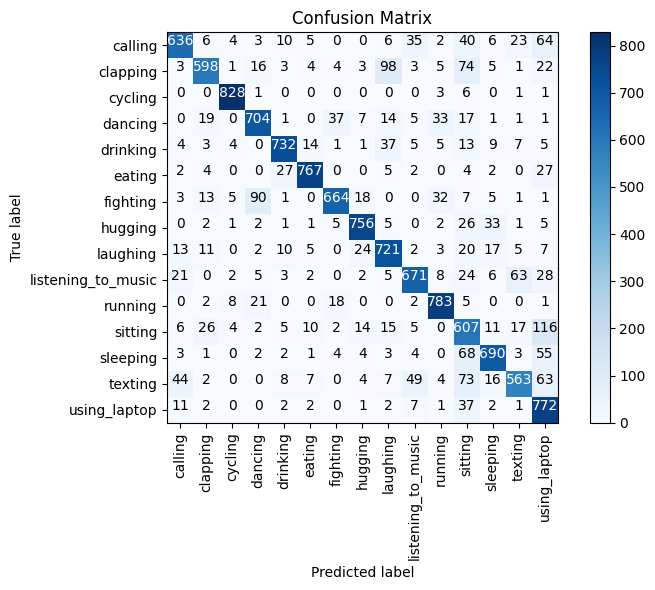
\includegraphics[width=0.5\textwidth]{./images/conf matrix had.png} 
    \caption{SligLIP 2 Confusion Matrix for Activity Classification}
    \label{fig:HAD-cm}
\end{figure}

% DO WE WANT THIS TO BE SUB- OR SUBSUB SECTION ????????????????????????????
\subsubsection{Fine-tuning}
Since the pre-trained model was not specifically trained for medication intake, fine-tuning was performed. This involved manual annotation of individual frames within the training set video. 


\section{Results}
\begin{figure}[H]
    \centering
    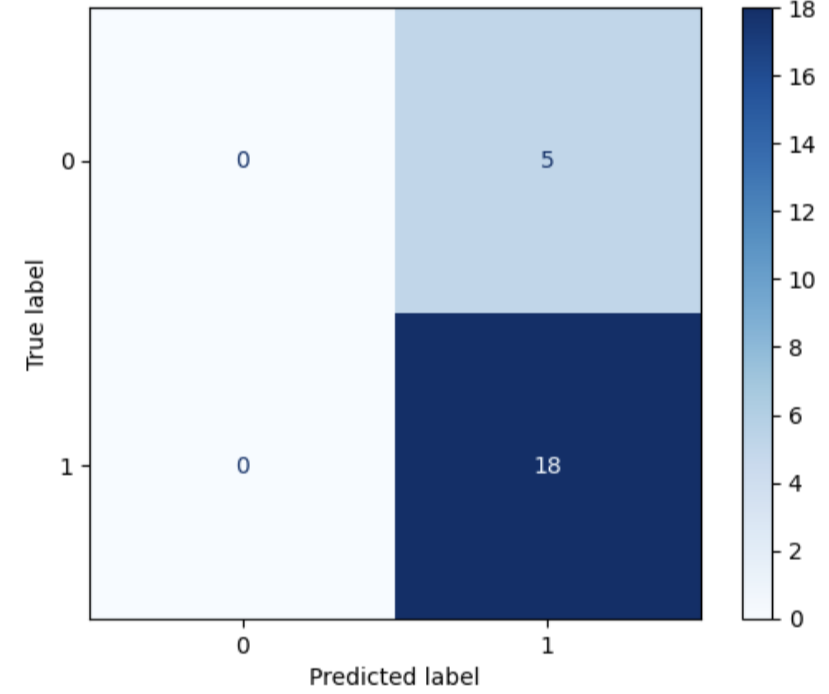
\includegraphics[width=0.5\textwidth]{./images/test confusion matrix.png} % Replace with your image file
    \caption{SligLIP 2 Confusion Matrix for Activity Classification}
    \label{fig:test-cm}
\end{figure}


% \section{Tables}
% You can include tables like this:

% \begin{table}[H]
%     \centering
%     \begin{tabular}{|c|c|c|}
%         \hline
%         Column 1 & Column 2 & Column 3 \
%         \hline
%         A & B & C \
%         1 & 2 & 3 \
%         \hline
%     \end{tabular}
%     \caption{Sample Table}
%     \label{tab:sample-table}
% \end{table}

\section{Conclusion}
Summarize the results and discuss the implications of your findings.

\section{Discussion and Recommendations}

\section*{References}

\end{document}
